Para la evaluación y comparación de los modelos entrenados con los
distintos hiperparámetros se recurrió a las mismas métricas que las
referidas en la sección \ref{subsection-results-features} al evaluar
los posibles vectorizadores.
\par
En este caso, se encontró que los hiperparámetros $C=0.1$ y $penalty=l2$
arrojaron los mejores valores promedios considerando las cinco iteraciones
de la validación cruzada. La única excepción a esto es el resultado en la
métrica de precisión, en el que el modelo entrenado con $C=2$ y $penalty=l2$
obtiene un mejor resultado. No obstante, este modelo muestra los valores
más bajos de cobertura y \textit{F1}. Es notable que, si bien tiene el mayor
valor de precisión observado, esto no llega a compensar su bajo rendimiento
en la cobertura y de ahí que también exhiba el valor de \textit{F1} más bajo.
Con valores más moderados, los demás modelos logran un mejor balance entre
\textit{precision} y \textit{recall} (ver tabla \ref{table-results-models-params}).

\begin{table}[h!]
    \centering
    \begin{adjustbox}{max width=\textwidth}
    \begin{tabular}{ *{7}{|c}| }
    \hline
    Parámetros & \textit{Accuracy} & Precisión & Cobertura & \textit{F1} & \textit{F1-macro} & \textit{F1-weighted} \\
    \hline\hline
    $C=0.1, penalty=l2$ & \cellcolor{highlight-blue!60}0.698 & 0.709 & \cellcolor{highlight-blue!60}0.786  & \cellcolor{highlight-blue!60}0.743 & \cellcolor{highlight-blue!60}0.686 & \cellcolor{highlight-blue!60}0.692 \\
    \hline
    $C=0.5, penalty=l2$ & 0.648 & 0.715 & 0.628  & 0.665 & 0.644 & 0.647 \\
    \hline
    $C=1, penalty=l2$ & \cellcolor{highlight-orange!60}0.622 & \cellcolor{highlight-orange!60}0.695 & 0.583 & 0.6310 & \cellcolor{highlight-orange!60}0.620 & \cellcolor{highlight-orange!60}0.622 \\
    \hline
    $C=2, penalty=l2$ & 0.629 & \cellcolor{highlight-blue!60}0.717 & \cellcolor{highlight-orange!60}0.560 & \cellcolor{highlight-orange!60}0.624 & 0.626 & 0.626 \\
    \hline
\end{tabular}
\end{adjustbox}
\caption{Resultados obtenidos tras evaluar un modelo de Regresión Logística con
distintos hiperparámetros. Los valores reflejan el rendimiento promedio de las
cinco iteraciones de la validación cruzada. Las celdas resaltadas en azul
corresponden a conjunto de hiperparámetros que obtuvo un mejor rendimiento
promedio en cada móetrica de evaluación y las resaltadas en naranja, al
que obtuvo el peor rendimiento.}
\label{table-results-models-params}
\end{table}

\begin{figure}[h!]
    \centering
    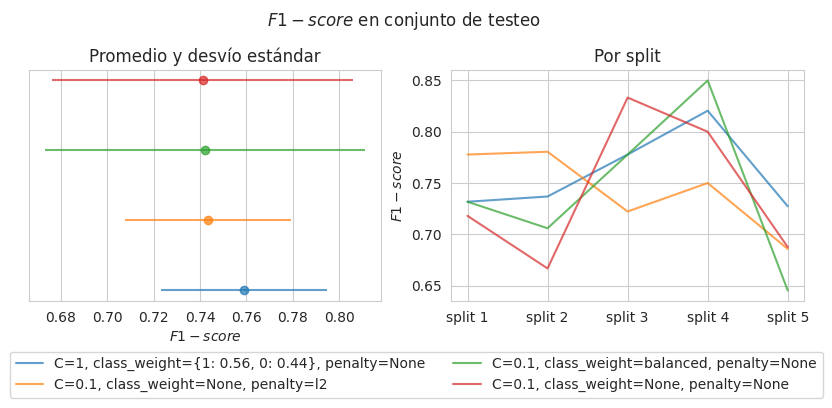
\includegraphics[scale=0.5]{../visualizations/parameters_selection/f1_by_split.png}
    \caption{Resultados obtenidos al evaluar los distintos modelos con
    \textit{F1} durante la validación cruzada. El gráfico a izquierda muestra el
    promedio y el desvió estándar de las cinco iteraciones para cada conjunto
    de hiperparámetros y el gráfico de la derecha compara los valores obtenidos en
    cada iteración.}
    \label{fig-results-models-f1}
\end{figure}

Adicionalmente, se graficó la media, el desvío estándar y el valor
obtenido en cada \textit{split} de la métrica \textit{F1}
para cada conjunto de hiperparámetros (ver figura \ref{fig-results-features-fit-time}).
Aquí podemos observar que los hiperparámetros $C=0.1$ y $penalty=l2$
no solo presenta una media mayor y desvío menor que los otros
conjuntos sino que, además, su rendimiento es mejor al resto en todas las
iteraciones, por lo que se optó por utilizar este como modelo final. Para ellos,
se lo reajustó con el conjunto completo de datos de entrenamiento y luego
se lo evaluó con el \textit{held-out} separado para este fin. La tabla
\ref{table-results-models-held-out} muestra los resultados obtenidos en
esta evaluación y la figura \ref{fig-results-models-held-out}, la matriz
de confusión resultante.

\begin{figure}
    \begin{minipage}[b]{.6\linewidth}
    \centering
        \begin{adjustbox}{max width=\textwidth}
        \begin{tabular}{ *{5}{|c}| }
        \hline
        Clase & Precisión & Cobertura & \textit{F1} & \textit{Soporte} \\
        \hline\hline
        0 (`en contra') & 0.80 & 0.67 & 0.73 & 18 \\
        \hline
        1 (`a favor') & 0.76 & 0.86 & 0.81  & 22 \\
        \hline\hline
        \textit{Accuray} & {--} & {--} & 0.78 & 40 \\
        \hline
        Promedio \textit{macro} & 0.78 & 0.77 & 0.77 & 40 \\
        \hline
        Promedio \textit{weighted} & 0.78 & 0.78 & 0.77 & 40 \\
        \hline
        \end{tabular}
        \end{adjustbox}
        \captionof{table}{Métricas de evaluación.}
        \label{table-results-models-held-out}
    \end{minipage}\hfill
    \begin{minipage}[t]{.35\linewidth}
      \centering
        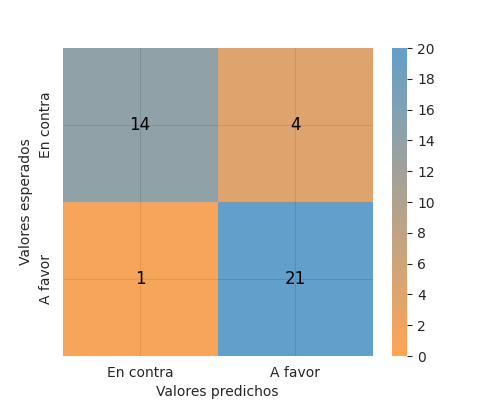
\includegraphics[scale=0.4]{../visualizations/models/confussion_matrix.png}
        \caption{Matriz de confusión.}
        \label{fig-results-models-held-out}
    \end{minipage}
    \caption*{Resultados obtenidos a partir de entrenar un modelo de
    Regresión Logística con los mejores hiperparámetros hallados
    ($C=0.1$ y $penalty=l2$) y el conjunto completo de datos de entrenamiento,
    y luego evaluarlo con el \textit{dataset} de testeo.}
  \end{figure}

Se observa que el modelo final obtuvo un mejor \textit{accuracy} que sus
versiones pre{--}entrenadas durante la validación cruzada. Posiblemente
esto se deba al incremento de los datos durante el entrenamiento.
Mientras que, en la selección de hiperparámetros, se entrenó con $127$ discursos
y se testeó con $32$ en cada iteración; en la versión final, el modelo fue entrenado
con $159$ documentos y evaluado con $40$. Este incremento no solo influye en
la cantidad y variabilidad de los datos que ve el modelo de regresión sino
también en el vectorizador, que se ve provisto de una mayor y más diversa fuente
de información para pesar las palabras presentes en los discursos y seleccionar
las $300$ más representativas de ambas clases a predecir.
\par
Al comparar las métricas de cobertura y precisión en la tabla
\ref{table-results-models-held-out}, se puede inferir que el modelo posee
una leve tendencia a predecir mayormente discursos `a favor': la cobertura
de esta clase es mayor, pero su precisión es menor; lo que indica que el modelo
predice mayormente esta clase aunque no en todos los casos acierta. Lo inverso
ocurre con los documentos `en contra'. Este fenómeno podría estar influido
por el hecho de tener clases levemente desbalanceadas y que sea la clase `a favor'
la mayoritaria.
\par
Por último, se graficó las $50$ palabras asociadas a los coeficientes positivos
y las $50$ asociadas a coeficientes negativos con mayor peso, aquellas que más
fuertemente conducen a predicciones de la clase `a favor' y `en contra' respectivamente.
La figura \ref{fig-results-models-feature-importance} nos permite conjeturar qué
\textit{tokens} caracterizan los discursos pertenecientes a ambas clases. Por el lado de los
discursos `a favor' se encuentran con \textit{tokens} como `mujer\_noun', `embarazo\_noun',
`sociedad\_noun', `salud\_noun', `respetar\_verb', `voluntaria\_adj', `integral\_adj',
`decidir\_verb', `autonomía\_noun' y `acompañamiento\_noun'. Y, por el lado de los
documentos `en contra', se ven `vida\_noun', `consitución\_noun', `norma\_noun',
`ley\_noun', `problema\_noun', `convicción\_noun', `humano\_adj', `niña\_noun'
\footnote{sjsjs}.

\begin{figure}[h!]
    \centering
    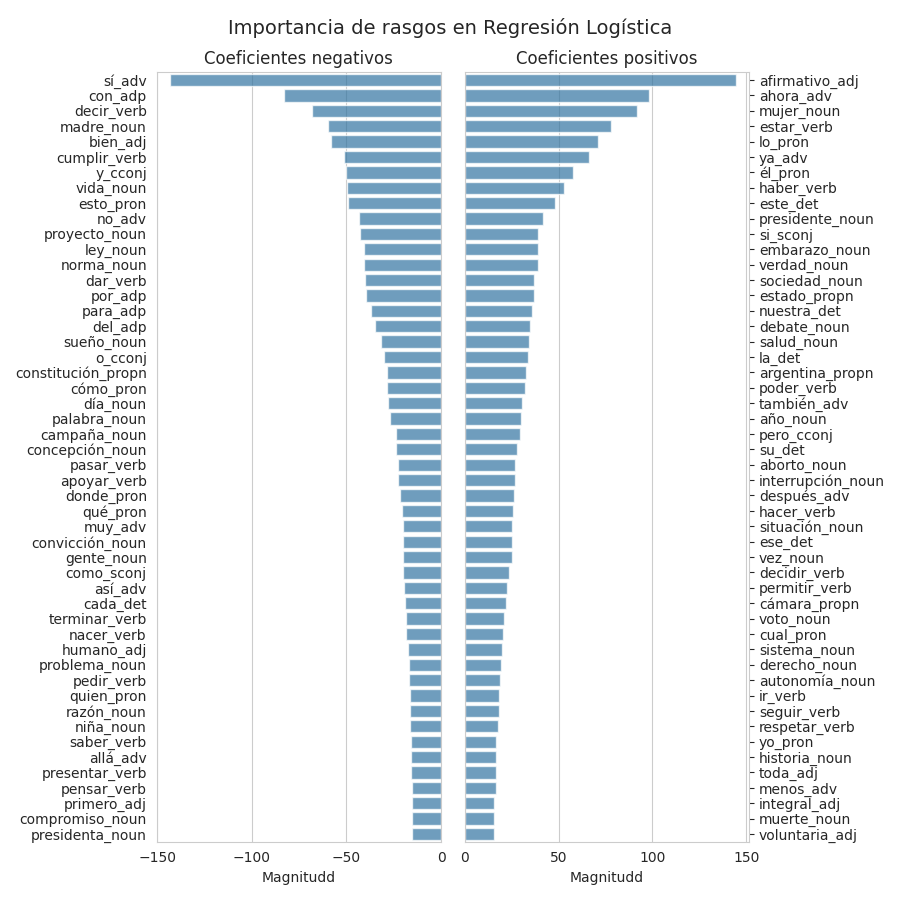
\includegraphics[scale=0.5]{../visualizations/models/lr_feature_importance_barplot_log_proba.png}
    \caption{Contraste}
    \label{fig-results-models-feature-importance}
\end{figure}